
\subsection{{\maxIdletime}が一般の場合}
\label{subsec:LineDifferentTimelimit}

全点の{\maxIdletime}が等しい場合は,
結局巡査がそれぞれ互いに素な区間を1つずつ担当する運行のみ考えればよいという
単純な状況になっていたが,
{\maxIdletime}が一般の場合は,
一部の頂点を複数の巡査が訪問して警備する必要がある場合が存在する.
%
図\ref{tikz:multiAgentExample2}(左)の例では,
中央の{\maxIdletime}の短い2つの頂点は2人の巡査に訪問されており,
また,全点の{\maxIdletime}が等しい場合に反して
各巡査の最適な運行はなんらかの区間の往復であるとは限らないことも分かる.


また,
この例では左の巡査は左端の点を{\maxIdletime}ちょうどごとに訪問しているが,
一方,図\ref{tikz:multiAgentExample2}(中央)の例では,
左側の巡査は左端の点をあえてより短い周期で訪問することで全点を警邏している.
図\ref{tikz:multiAgentExample2}(中央)と同じ入力に対して,
図\ref{tikz:multiAgentExample2}(右)のように左の巡査が
左端の点の{\maxIdletime}ぎりぎりの時間まで右の方へ動き左端へ帰る運行を行うと
2人の巡査がうまく協力できず全点の警備ができない.
このように,
補題\ref{lemm:LineEqualTimelimitIndependentInterval}のときのように
左端の点の{\maxIdletime}から順に巡査の運行を決定することも難しい例が存在する.

\begin{figure}[htbp]
  \centering
  \begin{tabular}{ccc}
  \begin{minipage}{0.32\hsize}
    \centering
    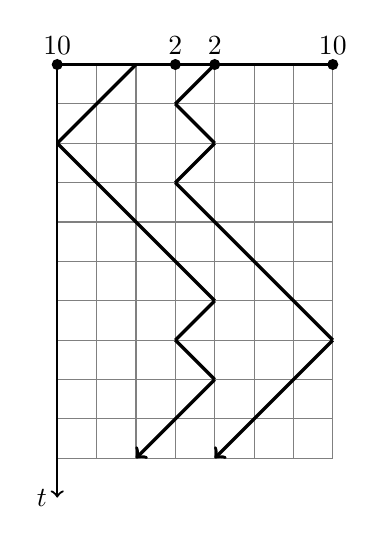
\begin{tikzpicture}
      \draw [help lines,thin,step=5mm] (0,-5.0) grid (3.5,0);
      \draw[thick] (0,0) -- (3.5,0) node [below] {};
      \draw[thick, ->] (0,0) -- (0,-5.5) node [left] {$t$};
      \fill ( 0   , 0) coordinate (c1) circle (2pt) node [above] {10};
      \fill ( 1.5 , 0) coordinate (c2) circle (2pt) node [above] {2};
      \fill ( 2.0 , 0) coordinate (c3) circle (2pt) node [above] {2};
      \fill ( 3.5 , 0) coordinate (c5) circle (2pt) node [above] {10};
      \draw[very thick,- ] ( 1.0, 0  )--(   0,-1.0);
      \draw[very thick,- ] (   0,-1.0)--( 2.0,-3.0);
      \draw[very thick,- ] ( 2.0,-3.0)--( 1.5,-3.5);
      \draw[very thick,- ] ( 1.5,-3.5)--( 2.0,-4.0);
      \draw[very thick,->] ( 2.0,-4.0)--( 1.0,-5.0);
      \draw[very thick,- ] ( 2.0, 0  )--( 1.5,-0.5);
      \draw[very thick,- ] ( 1.5,-0.5)--( 2.0,-1.0);
      \draw[very thick,- ] ( 2.0,-1.0)--( 1.5,-1.5);
      \draw[very thick,- ] ( 1.5,-1.5)--( 3.5,-3.5);
      \draw[very thick,->] ( 3.5,-3.5)--( 2.0,-5.0);
    \end{tikzpicture}
  \end{minipage}
  \begin{minipage}{0.32\hsize}
    \centering
    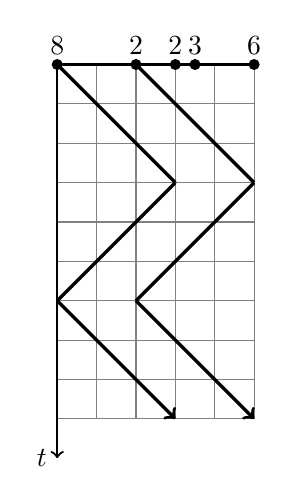
\begin{tikzpicture}
      \draw [help lines,thin,step=5mm] (0,-4.5) grid (2.5,0);
      \draw[thick] (0,0) -- (2.5,0) node [below] {};
      \draw[thick, ->] (0,0) -- (0,-5) node [left] {$t$};
      \fill ( 0   , 0) coordinate (c1) circle (2pt) node [above] {8};
      \fill ( 1   , 0) coordinate (c2) circle (2pt) node [above] {2};
      \fill ( 1.5 , 0) coordinate (c3) circle (2pt) node [above] {2};
      \fill ( 1.75, 0) coordinate (c4) circle (2pt) node [above] {3};
      \fill ( 2.5 , 0) coordinate (c5) circle (2pt) node [above] {6};
      \draw[very thick,- ] ( 0  , 0  )--( 1.5,-1.5);
      \draw[very thick,- ] ( 1.5,-1.5)--( 0  ,-3  );
      \draw[very thick,->] ( 0  ,-3  )--( 1.5,-4.5);
      \draw[very thick,- ] ( 1  , 0  )--( 2.5,-1.5);
      \draw[very thick,- ] ( 2.5,-1.5)--( 1  ,-3  );
      \draw[very thick,->] ( 1  ,-3  )--( 2.5,-4.5);
    \end{tikzpicture}
  \end{minipage}
  \begin{minipage}{0.32\hsize}
    \centering
    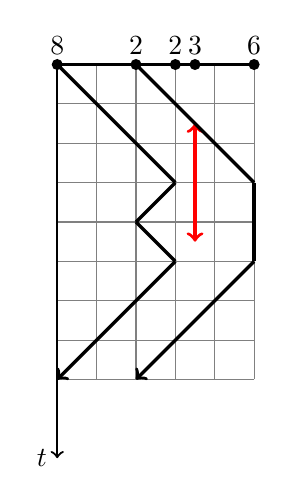
\begin{tikzpicture}
      \draw [help lines,thin,step=5mm] (0,-4) grid (2.5,0);
      \draw[thick] (0,0) -- (2.5,0) node [below] {};
      \draw[thick, ->] (0,0) -- (0,-5) node [left] {$t$};
      \fill ( 0   , 0) coordinate (c1) circle (2pt) node [above] {8};
      \fill ( 1   , 0) coordinate (c2) circle (2pt) node [above] {2};
      \fill ( 1.5 , 0) coordinate (c3) circle (2pt) node [above] {2};
      \fill ( 1.75, 0) coordinate (c4) circle (2pt) node [above] {3};
      \fill ( 2.5 , 0) coordinate (c5) circle (2pt) node [above] {6};
      \draw[very thick,red,<->] (1.75,-0.75)--(1.75,-2.25);
      \draw[very thick,- ] ( 0  , 0  )--( 1.5,-1.5);
      \draw[very thick,- ] ( 1.5,-1.5)--( 1  ,-2  );
      \draw[very thick,- ] ( 1  ,-2  )--( 1.5,-2.5);
      \draw[very thick,->] ( 1.5,-2.5)--( 0  ,-4  );
      \draw[very thick,- ] ( 1  , 0  )--( 2.5,-1.5);
      \draw[very thick,- ] ( 2.5,-1.5)--( 2.5,-2.5);
      \draw[very thick,->] ( 2.5,-2.5)--( 1  ,-4  );
    \end{tikzpicture}
  \end{minipage}
  \end{tabular}
  \caption{巡査の協力が必要な例.
    横軸を頂点の座標,縦軸を時刻として巡査の軌跡を表す.
    点の上の数値は{\maxIdletime}を表す.
    \ncomment{[あとで図を差し替える]}
    \label{tikz:multiAgentExample2}}
\end{figure}


これらの例は,{\maxIdletime}が異なる場合は巡査の運行を個別に決定するのは難しいということを示唆している.
しかしながら,この{\maxIdletime}が一般の場合での{\graphLine}上の{\patProb}の困難性を示すこともできなかった.
そこで,{\maxIdletime}より短い間隔で点を訪問しうることで運行の決定が複雑になる例が存在したことを踏まえて,
ここでは1章で定義した{\timeSpecifiedPatProbDecision}という別種の問題を代わりに考える.



グラフが{\graphLine}の場合の{\timeSpecifiedPatProbDecision}は次のようにも記述できる.

\begin{defi}
  $S \subset \Zset \times \Nset$とする.
  任意の$(t_1, x_1), (t_2, x_2) \in S$が
  $\abs{x_1 - x_2} \leq \abs{t_1 - t_2}$
  を満たすとき,$S$は運行可能であるという.
  また,分割$\{ P_1, \ldots, P_l \}$が運行可能であるとは,
  $P_1, \ldots, P_l$がそれぞれ運行可能集合であることである.
\end{defi}

任意の運行可能集合$S$に対して,
{\graphLine}上の巡査の運行$a$であって,
$S$のすべての元$(t, x)$に対して$a(t) = x$を満たす
(このとき$a$を運行可能集合$S$に対応する運行と呼ぶ)
ものが存在することは簡単に示すことができる.

\begin{timeSpecifiedPatrollingProblemOnLine}
巡査の人数を表す正の整数$m$
と$n$個の自然数の組$(q_i, r_i, x_i)_{ i \in \{ 1, \ldots, n \} }$が与えられる.
集合
$\{ (q_i k + r_i, x_i) \mid i \in \{1, \ldots, n\}, k \in \Zset \}$
を$m$個以下の運行可能集合に分割できるか判定せよ.
\end{timeSpecifiedPatrollingProblemOnLine}

\begin{theo}
\label{theo:LineTimeSpecifiedGreedy}
{\timeSpecifiedPatProbOnLine}を解く貪欲アルゴリズムが存在する.
\end{theo}


\begin{proof}[証明]
グラフが{\graphLine}の場合は順序保存運行を考えることができるのと同様に,
順序保存(運行可能)分割も考えることができる.
分割$\mathcal{P} = \{ P_1, \ldots, P_l \}$が順序保存であるとは,
$\mathcal{P}$に対応する運行$A = (a_1, \ldots, a_l)$であって
順序保存なものが存在することであり,
これは,
\[
  L(t, x)
    := \{ (t', x') \mid
          \abs{x - x'} > \abs{t - t'} \;\textrm{かつ}\; x' < x \}
     = \{ (t', x') \mid {x - x'} > \abs{t - t'} \}
\]
として,
任意の$P_i (i \in \{ 1 \ldots, l \})$について,
領域$\bigcup_{(t, x) \in P_i} L(t, x)$に
$P_j (i < j)$の点が存在しないことということもできる.

$X := \{ (q_i k + r_i, x_i) \mid i \in \{1, \ldots, n\}, k \in \Zset \}$
の任意の順序保存分割のうち一番左の集合は順序保存分割の定義から
$P_1 := \{ (t, x) \in X \mid L(t, x) \cap X = \emptyset \}$
の部分集合となる.
よって,$X$の最小の順序保存分割であって一番左の集合が
$P_1$であるようなものが存在する.
%
同様に,残りの$X \setminus P_1$の最小の順序保存分割であって一番左の集合が
$P_2 := \{ (t, x) \in X \setminus P_1 \mid L(t, x) \cap X \setminus P_1 = \emptyset \}$
であるようなものが存在する.
このように,集合$X$の左側から貪欲に運行可能集合を取り出していく操作を再帰的に繰り返すと,
最小の順序保存分割$\{ P_1, P_2, \ldots, P_l \}$が得られる.
これを$\mathfrak{P}(X)$と書くことにする.

以下では,集合$S \subseteq \Zset \times \Zset$に対して
$S[a:b) := \{ (t, x) \in S \mid a \leq t < b \}$
と定義する.

{\timeSpecifiedPatProbOnLine}の判定は$\card{\mathfrak{P}(X)} \leq m$が成り立つかの判定をすればよい.
$X$は無限集合であるから直接$X$を入力として分割$\mathfrak{P}(X)$を計算することはできないが,
この問題では$q_1, \ldots, q_n$が整数であることから
集合$X$は時刻(組$(t, x) \in X$の第1要素)について周期的である.
よって,
$\card{\mathfrak{P}(X)} \leq m$の判定は,
$T := lcm(q_1, \ldots, q_n)$として,
$X$の1周期分の有限部分集合$X[0:T)$を$\mathfrak{P}(X)$の一部となるように
(すなわち,$X[0:T)$を$\{ P_1[0:T), \ldots, P_l[0:T) \}$に)
分割し,$l \leq m$かどうか判定をすればよい.

有限集合$F$の分割$\mathfrak{P}(F)$を与える
{\setPartitionAlgorithm}は次のようになる.

\begin{setPartitionAlgorithmForTimeSpecifiedProblemOnLine}
入力を有限集合$F$とする.
初期値を$\mathcal{P} = \{\}$, $F' = F$とし,
$F' \neq \emptyset$である限り1.から3.を繰り返す.
\begin{enumerate}
\item $P \gets \{ (t, x) \in F' \mid L(t, x) \cap F' = \emptyset \}$
\item $\mathcal{P} \gets \mathcal{P} \cup \{ P \}$.
\item $F' \gets F' \setminus P$, 
\end{enumerate}
$\mathcal{P}$を出力する.
% $\blacksquare$
\end{setPartitionAlgorithmForTimeSpecifiedProblemOnLine}

前述の貪欲な分割の仕方で集合$S$から左端の運行可能集合
$s' := \{ (t, x) \in S \mid L(t, x) \cap S = \emptyset \}$
を取り出すときには,
定義の通り$s'$の任意の点$(t, x)$に対する領域$L(t, x)$に$S$の点が存在しないことのみが$s'$の点の条件である.
よって,
$\bigcup_{(t, x) \in X[0:T)} L(t, x)$を
{\setPartitionAlgorithm}の入力として与え,
出力された分割$\mathcal{P}$から$[0, T)$の範囲を取り出せば
$X[0:T)$の分割$\{ P_1[0:T), \ldots, P_l[0:T) \}$が得られる.
\end{proof}
